\documentclass[conference]{IEEEtran}
%\documentclass{sig-alternate-05-2015}
%\documentclass{article}
%\documentclass[10pt]{IEEEtran}
%\usepackage[cmex10]{amsmath}
%\usepackage[tight,footnotesize]{subFigure}
\usepackage{mdwmath}
%\bibliographystyle{IEEEtran}
%\bibliographystyle{acm}
\usepackage{mdwtab}
\usepackage{cite}
%\usepackage[dvipdfmx]{graphicx}
\usepackage{graphicx}
%\usepackage[numbers]{natbib}
\usepackage{notoccite}
%\usepackage[natbib=true,style=numeric,sorting=none]{biblatex}
\usepackage[...]{xcolor}
%\addbibresource{References}
\usepackage{listings}
\lstloadlanguages{C++,Pascal}

\usepackage[ampersand]{easylist}
\usepackage{times}
%\usepackage{mathtime}
\usepackage{booktabs}


\usepackage{color}
\usepackage[ampersand]{easylist}
\usepackage{times}
%\usepackage{mathtime}
\usepackage{booktabs}
\usepackage{listings}
\lstloadlanguages{C++,Pascal}

\usepackage{bmpsize}
\usepackage{epstopdf}
\usepackage{array}
\usepackage{caption}
\usepackage{subcaption}
\captionsetup{singlelinecheck=on}
\usepackage{multicol}
\usepackage{fancyhdr}
\pagenumbering{gobble}
\usepackage{lipsum}
\usepackage[english]{babel}
\usepackage{mathtools}
\usepackage[export]{adjustbox}
%\usepackage{amsmath}
\usepackage{MnSymbol}
\usepackage{wasysym}
\usepackage{mdframed}
\newcolumntype{x}[1]{>{\centering\arraybackslash\hspace{0pt}}p{#1}}
\usepackage{array}
%\usepackage{hyperref}
%\usepackage{geometry}
\usepackage[11pt]{moresize}


\newcolumntype{M}[1]{>{\centering\arraybackslash}m{#1}}
\newcolumntype{N}{@{}m{0pt}@{}}

\usepackage{balance}
\usepackage[export]{adjustbox}
\usepackage{epstopdf}
\usepackage{fixme}
\fxusetheme{color}
\fxsetup{
     status=draft,
     author=,
     layout=inline, % also try footnote or pdfnote
     theme=color
}


% Settings for the lstlistings environment
\lstset{
language=C++,                       % choose the language of the code
basicstyle=\footnotesize\ttfamily,  % the size of the fonts that are used for the
                                    % code
numbers=none,                       % where to put the line-numbers
numberstyle=\tiny,                  % the size of the fonts that are used for the
                                    % line-numbers
stepnumber=1,                       % the step between two line-numbers. If it's
                                    % 1 each line will be numbered
numbersep=5pt,                      % how far the line-numbers are from the code
%backgroundcolor=\color{gray},      % choose the background color. You must add
                                    % \usepackage{color}
showspaces=false,                   % show spaces adding particular underscores
showstringspaces=false,             % underline spaces within strings
showtabs=false,                     % show tabs within strings adding particular
                                    % underscores
keywordstyle=\bfseries\color{blue},  % color of the keywords
commentstyle=\color{purple},     % color of the comments
stringstyle=\color{red},        % color of strings
captionpos=b,                       % sets the caption-position to top
tabsize=2,                          % sets default tabsize to 2 spaces
frame=tb,                       % adds a frame around the code
breaklines=true,                    % sets automatic line breaking
breakatwhitespace=false,            % sets if automatic breaks should only happen
                                    % at whitespace
escapechar=\%,                      % toggles between regular LaTeX and listing
belowskip=0.3cm,                    % vspace after listing
morecomment=[s][\bfseries\color{blue}]{struct}{\ },
morecomment=[s][\bfseries\color{blue}]{class}{\ },
morecomment=[s][\bfseries\color{blue}]{public:}{\ },
morecomment=[s][\bfseries\color{blue}]{public}{\ },
morecomment=[s][\bfseries\color{blue}]{protected:}{\ },
morecomment=[s][\bfseries\color{blue}]{private:}{\ },
morecomment=[s][\bfseries\color{black}]{operator+}{\ },
xleftmargin=0.1cm,
%xrightmargin=0.1cm,
}

\definecolor{fxnote}{rgb}{0.8000,0.0000,0.0000}

\newcommand{\I}[1]{\textit{#1}}
\newcommand{\B}[1]{\textbf{#1}}
\newcommand{\T}[1]{\texttt{#1}}
\newcommand{\F}[1]{\B{\textcolor{red}{FIXME: #1}}}

\def\sharedaffiliation{%
\end{tabular}
\begin{tabular}{c}}

   
\begin{document}


%\setcopyright{acmcopyright}

%\doi{10.475/123_4}

% ISBN
%\isbn{123-4567-24-567/08/06}

%Conference
%\conferenceinfo{SPAA'28}{July 11--13, 2016, Asilomar State Beach, CL, USA}

%\acmPrice{\$15.00}

%
% --- Author Metadata here ---
%\conferenceinfo{WOODSTOCK}{'97 El Paso, Texas USA}

\title{HPX-Improving Parallel Applications Scalability for OP2}
\author{Zahra Khatami$^{1,2}$, Hartmut Kaiser$^{1,2}$ and J. Ramanujam$^{1}$ \\$^{1}$Center for Computation and Technology, Louisiana State University\\$^{2}$ The STE$||$AR Group, http://stellar-group.org
}
   
\maketitle

\begin{abstract}

Computer scientists and programmers face the difficultly in improving an application scalability while using the conventional techniques. So, advanced runtime system is required to take full advantage of the available parallel resources in order to achieve to the highest parallelism level as possible. In this paper we present the capability of HPX in achieving a desired scalability and allowing asynchronous task execution.

OP2 is an active library, which provides a framework of the parallel execution for unstructured grid applications on different multi-core/many-core hardware.  OpenMP is used for a loop parallelization within an application code generated with OP2 for both single-threaded and multi-threaded machines. We use HPX instead of OpenMP by porting the parallel simulation backend of OP2 to utilize HPX. We compare the performance results of different parallelization methods using HPX and OpenMP for a loop parallelization within an Airfoil application. The results of the strong scalability and the weak scaling tests for an Airfoil application on one node with up to 64 threads are presented, which show an improvement in OP2 parallelization performance while using HPX. 

Without changing OP2 API, we observe on an average by about 5\% scaling improvement in using \texttt{hpx::async} compared to \texttt{\#pragma omp parallel for}. To fully exploit the potentials of the emerging technology, we modify OP2 API to get a $future$ based model. We observe on an average by about 27\% scaling improvement in using \texttt{hpx::lcos::local::dataflow} compared to \texttt{\#pragma omp parallel for}. Our results shows the advantage of using asynchronous programming model implemented by HPX, which enables the better scalability due to the better latency hiding and using a fine-grain parallelism.




\end{abstract}

\begin{IEEEkeywords}
High Performance Computing, HPX, OP2, Asynchronous Task Execution.

\end{IEEEkeywords}

\section{Introduction}
Nowadays, a parallel application scalability is one of the major challenges when using the conventional techniques \cite{r11,r12}. To achieve an efficient scalability, it is needed to take full advantage of all available parallel resources. Avoiding resource starvation and hiding overheads can overcome this challenge and significantly improve a parallelism level. Parallelization is implemented with decomposing the domain space into several sub-domains and assigning each of them to the group of the processors. However, the overhead time due to the communication between processors inhibits the desired scalability. As a results, in addition to space, time should be considered as an another factor which helps to get a maximum possible parallelism level\cite{r7} \cite{r14}. So the parallelization should be done in both space and time domains. 

HPX \cite{r19} overcomes this difficulty by significantly reducing the SLOW factors \cite{r6}. SLOW factors avoid the parallel scalability, which are explained as: Starvation, which is due to the poor utilization of resources; Latencies, which is the related delay for accessing to the remote resources; Overhead, which is the cost for managing parallel actions; Waiting, which is the related delay due to the shared resources \cite{r7}. 

HPX is a parallel C++ runtime system that aims to use the full parallelization capabilities of today's and tomorrow's hardware available for an application. HPX implements the concepts of the ParalleX execution model \cite{o9,o10,o11} on conventional systems including Windows, Macintosh, Linux clusters, XeonPhi, Bluegene/Q and the Android. HPX enables asynchronous task execution which results in having a parallelization in both space and time domains. As a result, it removes a global barrier synchronization and improves a parallel performance. In this paper, HPX is used to improve a performance of OP2 for a parallel application scalability.

Op2 provides a framework of the parallel execution for unstructured grid applications \cite{o1}. OP2's design and development is presented in \cite{o2,o12}. With Op2, applications can be targeted to execute on different multi-core/many-core hardware \cite{o2,o3}. To achieve further performance gains with OP2 on modern multi-core/many-core hardware, some optimizations should be applied to improve performance for different parallel applications. This can be obtained by avoiding the SLOW factors as much as possible. OpenMP is used for a loop parallelization in OP2 on a single node and also on the distributed nodes using MPI. \texttt{\#pragma omp parallel for} used for a loop parallelization in OP2 causes an implicit global barrier at the end of loop, which does not result in an efficient speedup. Using HPX parallelization methods instead of OpenMP helps eliminating these SLOW factors and extracting an optimal parallelism from a parallel application.

This paper describes the results from porting the parallel simulation backend of OP2 to utilize HPX. We study the parallelization performance of OP2 with HPX with both changing OP2 API and without changing OP2 API. The parallelization performance is studied on a standard unstructured mesh finite volume computational fluid dynamics (CFD) application, called Airfoil, which uses OP2 API and it is written in C$++$. The experimental results of an application scalability are studied while using HPX in OP2 for a loop parallelization and these results are compared with OpenMP performance.

The remainder of this paper is structured as following: Section \ref{sec:op2} explains briefly about OP2. An overview of the HPX is presented in Section \ref{sec:hpx} with the key features that distinguish it from the conventional techniques. Section \ref{sec:air} presents the Airfoil application used in this research and gives details of using HPX for loop parallelization used in OP2. The experimental tests and the strong scaling are presented in Section \ref{sec:res}. Conclusion is provided in Section \ref{sec:future}.

\section{OP2}
\label{sec:op2}

This paper presents an optimization study of the OP2 ``active" library \cite{o1}. OP2 utilizes the source-to-source translation which targets a single application code to be written for different backend hardware platforms \cite{o2,o3,o4}. OP2 generates a code for single-threaded on a CPUs, multi-threaded using OpenMP for single SMP node of multi-core CPUs, using CUDA for a single NVIDIA GPU, using MPI and OpenMP for a cluster of CPUs and using MPI and CUDA for a cluster of NVIDIA GPUs \cite{o4}. 

OP2 API has been developed for an unstructured grids. So the algorithm includes four different parts: sets, data on sets, mapping connectivity between the sets and computation on the sets \cite{o2,o7}. Sets can be nodes, edges, faces or other elements. Data are values and parameters associated with these sets. Map is used to define a connectivity between sets. The operation over a set is done with a user's defined kernel function within a loop. Arguments passed to loops in OP2 have an explicit indication that how each of them are accessed within a loop : \texttt{OP\_READ} (read only), \texttt{OP\_WRITE} (write) or \texttt{OP\_INC} (increment - to avoid race conditions due to indirectly accessed) \cite{o1}. There is two different kinds of $loops$ defined in OP2: $indirect$ loop and $direct$ loop. If data is accessed through a mapping, the loop is an $indirect$ loop. Otherwise, it is a $direct$ loop. 

In this research Airfoil application is studied that is presented in \cite{o8}. We demonstrate OP2 loops through the C$++$ code shown in Figure \ref{o1}, which includes \texttt{op\_par\_loop\_save\_soln} and \texttt{op\_par\_loop\_adt\_calc} loops from an Airfoil application. \texttt{op\_par\_loop\_save\_soln} loop is a $direct$ loop which applies \texttt{save\_soln} over cells with accessing data arguments \texttt{p\_q} and \texttt{p\_qold} passed to the loop. \texttt{op\_par\_loop\_adt\_calc} is an $indirect$ loop which applies \texttt{op\_par\_loop\_adt\_calc} over cells with accessing data arguments \texttt{p\_x}, \texttt{p\_q} and \texttt{p\_adt} passed to the loop. Function \texttt{op\_arg\_dat} creates an argument based on the information passed to it. For example, in \texttt{op\_arg\_dat(p\_x,0,pcell,2,"double",OP\_READ)}, an argument is created from its inputs, where \texttt{p\_x} is a data, $0$ shows that a data is accessed indirectly, \texttt{pcell} is a map which a data is mapped on, $2$ is a dimension of data, \texttt{double} shows a type of data and \texttt{OP\_READ} shows that this data is a read\_only data.

\begin{figure} 
    \begin{lstlisting}
op_par_loop_save_soln("save_soln", cells,
  op_arg_dat(p_q,-1,OP_ID,4,"double",OP_READ),
  op_arg_dat(p_qold,-1,OP_ID,4,"double",OP_WRITE));
  
op_par_loop_adt_calc("adt_calc",cells,
  op_arg_dat(p_x,0,pcell,2,"double",OP_READ),
  op_arg_dat(p_x,1,pcell,2,"double",OP_READ),
  op_arg_dat(p_x,2,pcell,2,"double",OP_READ),
  op_arg_dat(p_x,3,pcell,2,"double",OP_READ),
  op_arg_dat(p_q,-1,OP_ID,4,"double",OP_READ),
  op_arg_dat(p_adt,-1,OP_ID,1,"double",OP_WRITE));
  
    \end{lstlisting}
    \caption{\small{\texttt{op\_par\_loop\_save\_soln} and \texttt{op\_par\_loop\_adt\_calc} loops from an Airfoil application.  \texttt{op\_par\_loop\_save\_soln} loop is a $direct$ loop and \texttt{op\_par\_loop\_adt\_calc} is an $indirect$ loop.}}
    \label{o1}
\end{figure}



OP2's design is based on achieving a near-optimal performance for scaling on multi-core processors. In \cite{o3,o4}, it is studied that OP2 API is able to produce a near-optimal performance in a parallel loops for different frameworks without the intervention of the application programmer. However, processors starvation, latencies and overhead communications in parallelization using conventional techniques usually inhibits a desired scalability. Most of the conventional parallelization methods are based on the fork-join model. In the fork-join model, the computational process will be stopped if the results from the previous step are not completed yet. As a result, there is always a global barrier after each step. 

\texttt{\#pragma omp parallel for} is used in a code generated with OP2 for a single-threaded and also for a multi-threaded machine. There is an implicit global barrier using \texttt{\#pragma omp parallel for}, which avoids extracting an optimal parallelism from a parallel application. In this research, HPX is used for loop parallelization instead of using OpenMP.  HPX allows automatically creating an execution tree of an application which represents a dependency graph. This enables HPX to have an asynchronous task execution. The performance of HPX is explained in more details in section \ref{sec:hpx}.                                                                                                                                                                                                                                                                                                                                                                                                                                                                                                                                                                                                                                                                                                                                                                                                                            


An Airfoil application includes both $direct$ and $indirect$ loops that all of them are parallelized with OpenMP. Optimization of Airfoil application with HPX for parallelizing loops used in a code generated with OP2 is discussed in more details in section \ref{sec:air}. The source-to-source code translator for OP2 is written in Matlab and Python \cite{o3}. Python source-to-source code translator is used in this research and some part of it is modified to automatically generate the parallel loops with HPX instead of OpenMP within an application problem. 


\section{HPX}
\label{sec:hpx}

In order to hide latencies even for very short operations, having a light-weight threads is needed which should have the extremely short context switching times, that results in becoming optimally executable within one cycle. HPX is a parallel C++ runtime system that facilitates distributed operations and enables fine-grained task parallelism. The fine-grained tasks result in better load balancing and lower communication overheads. HPX has been developed  to overcome conventional limitations such as global barriers and poor latency hiding \cite{r6} by embracing a new way of coordinating parallel execution. It has been developed for different architectures, such as large Non Uniform Memory Access (NUMA) machines, SMP nodes and systems using Xeon Phi accelerators.


HPX's design focuses on parallelism than concurrency. Concurrency is defined to have several simultaneously computations and parallelism is simultaneous execution of tasks\cite{r15}. So it enables HPX to have both time and spatial parallelization \cite{r19} due to using \textit{$future$}, which results in having asynchronous task execution. In HPX, asynchronous function execution is the fundamental basic of asynchronous parallelism.

A \textit{$future$} is a computational result that is initially unknown but becomes available at a later time~\cite{r20}. The goal of using \textit{$future$} is to let every computation proceed as far as possible. Using \textit{$future$} enables the continuation of the process without waiting for the results of the previous step to be completed, which eliminates the global barriers at the end of the execution of the parallel loop. \textit{$future$} based parallelization provides rich semantics for exploiting the higher level parallelism available within each application that significantly improves scaling. Figure~\ref{f4} shows the scheme of \textit{$future$} performance with 2 \textit{localities}, where a \textit{locality} is a collection of processing units (PUs) that have access to the same main memory. 


\begin{figure} [!h]
\captionsetup{justification=centering}
\begin{center}
\centering
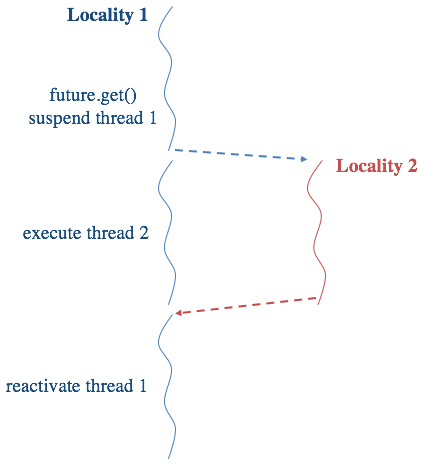
\includegraphics[width=0.75\columnwidth]{Pictures/f4a.jpg}
\caption {The principle of operation of a \textit{$future$} in HPX}
\label{f4}
\end{center}
\end{figure}



Figure~\ref{f4} shows that until returning the computed value, the other threads do not stop their process. Instead, they continue their process until they need the computation result from the previous step. Then, HPX threads requesting suspend until $future$ value is computed. Threads access the $future$ value by performing a \textit{$future$.get()} in Figure~\ref{f4}. When the result becomes available, the \textit{$future$} resumes all HPX suspended threads waiting for the value. It can be seen that this process eliminates the global barrier synchronizations at the end of application parallelization while only those threads that depend on the $future$ value are suspended. With this scheme, HPX allows asynchronous execution of threads.


\section{Airfoil code with HPX}
\label{sec:air}

For our evaluation we chose the Airfoil application presented in \cite{o8}. This model uses an unstructured grid and it consists of five parallel loops: \texttt{op\_par\_loop\_save\_soln}, \texttt{op\_par\_loop\_adt\_calc}, \texttt{op\_par\_loop\_res\_calc}, \texttt{op\_par\_loop\_bres\_calc}, \texttt{op\_par\_loop\_update}, which \texttt{op\_par\_loop\_save\_soln},  and \texttt{op\_par\_loop\_update} loops are $direct$ loops and the others are $indirect$ loops. Figure \ref{l1} shows the sequential loops used in Airfoil application within \texttt{airfoil.cpp}. Saving old data values, applying the computation on each data value and updating them are implemented with these five loops. Each loop iterates over a specified set and the operations that is performed with a user's kernels defined in a header file for each loop: \texttt{save\_soln.h}, \texttt{adt\_calc.h}, \texttt{res\_calc.h}, \texttt{bres\_calc.h} and \texttt{update.h}.  OP2 API provides a parallel loop function allowing the computation over sets through \texttt{op\_par\_loop} for each loops in Figure \ref{l1}. 

\begin{figure} [!h]
    \begin{lstlisting}
op_par_loop_save_soln("save_soln", cells,
  op_arg_dat(data_a0,...),...,
  op_arg_dat(data_an);
  
op_par_loop_adt_calc("adt_calc",cells,
  op_arg_dat(data_b0,...,
  op_arg_dat(data_bn);
  
op_par_loop_res_calc("res_calc",edges,
  op_arg_dat(data_c0,...,
  op_arg_dat(data_cn);

op_par_loop_bres_calc("bres_calc",bedges,
  op_arg_dat(data_d0,...,
  op_arg_dat(data_dn);
  
op_par_loop_update("update",cells,
  op_arg_dat(data_e0,...,
  op_arg_dat(data_en);
  
    \end{lstlisting}
    \caption{\small{Five loops are used in \texttt{airfoil.cpp} for saving old data values, applying the computation on each data value and updating them. \texttt{save\_soln} and \texttt{update} loops are $direct$ loops and the others are $indirect$ one.}}
    \label{l1}
\end{figure}


Figure \ref{l2} shows the loop of \texttt{op\_par\_loop\_adt\_calc} function from Figure \ref{l1} parsed with OP2, which illustrates how each cell updates its data value with using \texttt{blockId}, \texttt{offset\_b} and \texttt{nelem}. The value of \texttt{blockId} is defined based on the value of \texttt{blockIdx} captured from OP2 API.  \texttt{offset\_b} and \texttt{nelem} are computed based on the value of \texttt{blockId}. The arguments are passed to the \texttt{adt\_calc} user kernel subroutine, which does the computation for each iteration in the inner loop from \texttt{offset\_b} to \texttt{offset\_b+nelem} of each iteration of the outer loop from \texttt{0} to \texttt{nblocks}. More details about the Airfoil application and its computation process can be found in \cite{o8}.

\begin{figure} [!h]
    \begin{lstlisting}
#pragma omp parallel for
for(int blockIdx=0; blockIdx<nblocks; blockIdx++){
  int blockId  = //defined with blockIdx in OP2 API
  int nelem    = //defined based on blockId 
  int offset_b = //defined based on blockId
        
  for ( int n=offset_b; n<offset_b+nelem; n++ ){
   .
   .
   .

   adt_calc(...);
  }
}
  
    \end{lstlisting}
    \caption{\small{\texttt{\#pragma omp parallel for} is used for loop parallelization in OP2 for Airfoil application to obtain the loop parallelization on one node and also on the distributed nodes using MPI.}}
    \label{l2}
\end{figure}


As shown in Figure \ref{l2}, \texttt{\#pragma omp parallel for} is used for each loops passed with \texttt{op\_par\_loop} in OP2 for parallelizing the loops on one node and also on distributed nodes. However, scalability is limited due to the sequential time caused by an implicit barrier in the fork-join model \cite{r23} between the parallel loops as described by Amdahl's Law. HPX parallelization methods are used here instead of OpenMP to achieve an optimal parallelization for parallelizing the loops parsed with OP2. 

In this research we use different HPX parallelization methods without changing OP2 API and with changing OP2 API. Airfoil parallelization performance with HPX and without changing OP2 API is studied in Section \ref{sec:without} and with the modified OP2 API is studied in Section \ref{sec:with}. The comparison results of these two methods and OpenMP can be found in section \ref{sec:res}.

\subsection{\textbf{HPX without changing OP2 API}}
\label{sec:without}

In this Section, we study two different HPX parallelization methods on an Airfoil application without changing the OP2 API. In Section \ref{sec:for}, \texttt{parallel::for\_each} with \texttt{hpx::parallel::par} as an execution policy is used for parallelizing both $direct$ and $indirect$ loops. In Section \ref{sec:async}, \texttt{hpx::async} and \texttt{hpx::parallel::for\_each} with \texttt{hpx::parallel::par} is used for parallelizing the $direct$ loops, and for the $indirect$ loops, \texttt{hpx::parallel::for\_each} with \texttt{hpx::parallel::par(task)} as an execution policy is implemented . 



\subsubsection{\textbf{\texttt{parallel::for\_each}}}
\label{sec:for}

In this method, we implement one of the execution policies of HPX to make the loops shown in Figure \ref{l1} executing in parallel. The list of the execution policies can be found in \cite{hpx_v0.9.11}. 

\texttt{hpx::parallel::par} as an execution policy is used while implementing \texttt{hpx::parallel::for\_each}. We were able to modify OP2 source-to-source translator with Python to automatically produce \texttt{hpx::parallel::for\_each} instead of using \texttt{\#pragma omp parallel for} for a loop parallelization. In this method \texttt{airfoil.cpp} remains the same as Figure \ref{l1} and also OP2 API is not changed too.

\begin{figure} 
    \begin{lstlisting}    
auto r=boost::irange(0, nblocks);
hpx::parallel::for_each(hpx::parallel::par,
  r.begin(), r.end(),[&](std::size_t blockIdx){
  
  int blockId  = //defined with blockIdx in OP2 API
  int nelem    = //defined based on blockId 
  int offset_b = //defined based on blockId
        
  for ( int n=offset_b; n<offset_b+nelem; n++ ){
   .
   .
   .

   adt_calc(...);
  }
});
  
    \end{lstlisting}
    \caption{\small{Implementing \texttt{hpx::parallel::for\_each} for loop parallelization in OP2 for Airfoil application. HPX is able to control a grain size in this method. As a result, it helps in reducing processor starvation caused by the fork-join barrier at the end of the execution of the parallel loop.}}
    \label{l3}
\end{figure}

\begin{figure} 
    \begin{lstlisting}    
hpx::parallel::dynamic_chunk_size dcs(SIZE);
auto r=boost::irange(0, nblocks);
hpx::parallel::for_each(hpx::parallel::par.with(dcs),r.begin(),r.end(),[&](std::size_t blockIdx){
  
  int blockId  = //defined with blockIdx in OP2 API
  int nelem    = //defined based on blockId 
  int offset_b = //defined based on blockId
        
  for ( int n=offset_b; n<offset_b+nelem; n++ ){
   .
   .
   .

   adt_calc(...);
  }
});
  
    \end{lstlisting}
    \caption{\small{Implementing \texttt{hpx::parallel::for\_each} for loop parallelization in OP2 for Airfoil application. HPX is able to avoid degrading the scalability for small loops with defining a static grain size with \texttt{hpx::parallel::dynamic\_chunk\_size dcs(SIZE)} before the parallel loop execution.}}
    \label{l3b}
\end{figure}



This example exposes the same disadvantage as OpenMP, which is the representation of fork-join parallelism that introduces the global barriers at the end of the loop. But the difference of this method with OpenMP is that with using \texttt{hpx::parallel::for\_each}, HPX is able to automatically control a grain size during a runtime. Grain size is the amount of works per threads. As discussed in section \ref{sec:hpx}, HPX enables fine-grained task parallelism and determines the grain size as small as possible to give task to all available threads. Grain size, which is named as \texttt{chunk\_size} within HPX, is determined from auto-partitioner algorithm in HPX estimated at runtime while sequentially executing $1\%$ of an application. So \texttt{hpx::parallel::for\_each} helps creating sufficient amount of parallelism that how many iterations will run on the same thread, which helps in reducing processor starvation caused by the fork-join barrier at the end of the execution of the parallel loop.  Figure \ref{l3} shows the loop of \texttt{op\_par\_loop\_adt\_calc} function parsed with OP2 with dynamic \texttt{chunk\_size}. 

However, it should be considered that if the computational time of a loop is not large enough compared to an application execution time, using an auto-partitioner algorithm within HPX will not be efficient. Since for the small loops, $1\%$ of an application execution time used for determining a grain size will affect the application's scalability, so HPX provides another way to avoid degrading the scalability while using \texttt{hpx::parallel::for\_each}. Grain size can be determined as a static grain size with \texttt{hpx::parallel::for\_each(par.with(dcs))} before executing a loop, which \texttt{dcs} is defined with \texttt{hpx::parallel::dynamic\_chunk\_size dcs(SIZE)} as a static size.  Figure \ref{l3b} shows the loop of \texttt{op\_par\_loop\_adt\_calc} function with static \texttt{chunk\_size} implemented with \texttt{hpx::parallel::dynamic\_chunk\_size dcs(SIZE)}. The experimental result for an Airfoil application is discussed in section \ref{sec:res} for both dynamic and static \texttt{chunk\_size}.

\subsubsection{\textbf{\texttt{async} and \texttt{parallel::for\_each}}}
\label{sec:async}

Here, we implement two different parallelization methods for the loops based on their types. For the $direct$ loops, \texttt{hpx::async} and \texttt{hpx::parallel::for\_each} with \texttt{hpx::parallel::par} as an execution policy is used. For  the $indirect$ loops,  \texttt{hpx::parallel::for\_each} with \texttt{hpx::parallel::par(task)} as an execution policy is implemented. The call to \texttt{hpx::async} and also \texttt{hpx::parallel::par(task)} provide a new $future$ instance, which represents the result of the function execution that make the invocation of the loop asynchronous. Asynchronous task execution means that a new HPX-thread will be scheduled. 

In Figure \ref{l6}, \texttt{hpx::async} and \texttt{hpx::parallel::for\_each} with \texttt{hpx::parallel::par} is used for \texttt{op\_par\_loop\_save\_soln}, which is a $direct$ loop and returns a $future$ representing the result of a function. In Figure \ref{l6b},  \texttt{hpx::parallel::for\_each} with \texttt{hpx::parallel::par(task)} is used for \texttt{op\_par\_loop\_adt\_calc}, which is an $indirect$ loop and it also returns a $future$ representing the result of a function. The $future$ returned from all $direct$ and $indirect$ loops allow the asynchronization for the executed loops.

\begin{figure} 
    \begin{lstlisting}    

return async(hpx::launch::async,[adt_calc,set,arg0,...,argn1](){

    hpx::parallel::dynamic_chunk_size dcs(SIZE);
    auto r=boost::irange(0, nthreads);
    hpx::parallel::for_each(hpx::parallel::par.with(dcs), r.begin(), r.end(),[&](std::size_t thr){
  
    int start  = //defined based on number of threads;
    int finish =//defined based on number of threads;
        
    for ( int n=start; n<finish; n++ ){
     save_soln(...);
    }
  });
  
    \end{lstlisting}
    \caption{\small{Implementing \texttt{hpx::async} and \texttt{hpx::parallel::for\_each} with \texttt{hpx::parallel::par} for a $direct$ loop parallelization in OP2 for Airfoil application. The returned $future$ representing the result of a function.}}
    \label{l6}
\end{figure}


\begin{figure} 
    \begin{lstlisting}    
hpx::parallel::dynamic_chunk_size dcs(SIZE);
auto r=boost::irange(0, nblocks);
hpx::future<void> new_data;
new_data=hpx::parallel::for_each(hpx::parallel::par(hpx::parallel::task).with(dcs), r.begin(), r.end(),[&](std::size_t blockIdx){
  
  int blockId  = //defined with blockIdx in OP2 API
  int nelem    = //defined based on blockId 
  int offset_b = //defined based on blockId
        
  for ( int n=offset_b; n<offset_b+nelem; n++ ){
   .
   .
   .

   adt_calc(...);
  }
});
  
    \end{lstlisting}
    \caption{\small{Implementing \texttt{hpx::parallel::for\_each} with \texttt{hpx::parallel::par(task)} for an $indirect$ loop parallelization in OP2 for Airfoil application. The returned $future$ representing the result of a function.}}
    \label{l6b}
\end{figure}

\begin{figure} [!h]
    \begin{lstlisting}   

new_data1=op_par_loop_save_soln("save_soln",
   cells,op_arg_dat_0,...,op_arg_dat_n1);
  
new_data2=op_par_loop_adt_calc_("adt_calc",
   cells,op_arg_dat_0,...,op_arg_dat_n2);
   
new_data3=op_par_loop_res_calc("res_calc",
   edges,op_arg_dat_0,...,op_arg_dat_n3);
 
new_data4=op_par_loop_bres_calc("bres_calc",
   bedges,op_arg_dat_0,...,op_arg_dat_n4);
   
new_data1.get();
new_data2.get();  
 
new_data5=op_par_loop_update("update",
   cells,op_arg_dat_0,...,op_arg_dat_n5);

new_data3.get();
new_data4.get();
new_data5.get();

    
    \end{lstlisting}
    \caption{\small{\texttt{airfoil.cpp} is changed while using \texttt{hpx::async} and \texttt{hpx::parallel::par(task)} for loop parallelization in OP2. \texttt{new\_data} is returned from each kernel function after calling \texttt{op\_par\_loop} and \texttt{new\_data.get()} is used to get $futures$ ready before the next steps.}}
    \label{l4}
\end{figure}


In this method OP2 API is not changed but \texttt{airfoil.cpp} is changed as shown Figure \ref{l4}. Each kernel function within \texttt{op\_par\_loop} returns a $future$ stored in a \texttt{new\_data}. Each future depends on a future in a previous step. So, \texttt{new\_data.get()} is used to get all $futures$ ready before the next steps. The place of using \texttt{new\_data.get()} depends on an application and a programmer should put them manually in a right place by considering the data dependency between loops. OP2 source-to-source translator with Python is modified and it automatically produces \texttt{hpx::async} and \texttt{hpx::parallel::for\_each} with \texttt{hpx::parallel::par} for each direct loops and \texttt{hpx::parallel::for\_each} with \texttt{hpx::parallel::par(task)} for each $indirect$ loops within Airfoil application. The experimental results of this section can be found in Section \ref{sec:res}.



\subsection{\textbf{HPX with the modified OP2 API}}
\label{sec:with}

To fully exploit the potentials of the emerging technology, we modify OP2 API to get a $future$ based model. As shown in Figure \ref{o1}, \texttt{op\_arg\_dat} creates an argument which is passed to a function through \texttt{op\_par\_loop}. The modified OP2 API passes the argument as a $future$, which is created with the modified \texttt{op\_arg\_dat} shown in Figure \ref{o2}. Here, we implement \texttt{hpx::lcos::local::dataflow} in \texttt{op\_arg\_dat}, which gives an argument as a $future$ whenever the data (\texttt{dat}) of an argument becomes ready. In using \texttt{hpx::lcos::local::dataflow}, if an argument is a $future$, then the invocation of a function will be delayed. Non-future arguments are passed through. For an instance, in Figure \ref{o2}, \texttt{dat} expressed at the last line of the code invokes a function only once this future gets ready. \texttt{unwrapped} is a helper function created in HPX, which unwraps the futures for a function and passes along the actual results. All these $future$ arguments are passed to a function within each \texttt{op\_par\_loop}.

\begin{figure}
    \begin{lstlisting}    
using hpx::lcos::local::dataflow;
using hpx::util::unwrapped;    

return dataflow(unwrapped([&](op_dat dat){
     .
     . //same as op_arg_dat in an original OP2 API
     .

    return arg;
    }
  }),dat);
  
    \end{lstlisting}
    \caption{\small{\texttt{op\_arg\_dat} is modified to create an argument as a $future$, which is passed to a function through \texttt{op\_par\_loop}.}}
    \label{o2}
\end{figure}

\texttt{hpx::lcos::local::dataflow} with \texttt{hpx::parallel::for\_each} is implemented for a loop parallelization that makes the invocation of the loop asynchronous. In Figure \ref{l3b}, \texttt{hpx::lcos::local::dataflow} returns a $future$ representing the result of a function and allows the asynchronization for the executed loops. All arguments passed to each kernel functions are $future$ except the name of a function and \texttt{op\_set} passed to a loop. \texttt{hpx::parallel::for\_each} as a previous method (see section \ref{sec:air}) is used for a loop parallelization within each kernels. It should be noted that the function represented in this section is the same as a function in section \ref{sec:for} but asynchronous. The $future$s returned represent the results as a dependency tree, which represents the execution graph that is automatically created. As a result, a modified OP2 API and \texttt{hpx::lcos::local::dataflow} give an ability of having an asynchronous task execution. 


\begin{figure}
    \begin{lstlisting}    
using hpx::lcos::local::dataflow;
using hpx::util::unwrapped;    

return dataflow(unwrapped([&adt_calc,set](set, op_arg arg0, ... , op_arg argn2){

    hpx::parallel::dynamic_chunk_size dcs(SIZE);
    auto r=boost::irange(0, nblocks);
    hpx::parallel::for_each(hpx::parallel::par.with(dcs), r.begin(), r.end(),[&](std::size_t blockIdx){
  
    int blockId  = //defined with blockIdx in OP2
    int nelem    = //defined based on blockId 
    int offset_b = //defined based on blockId
        
    for ( int n=offset_b; n<offset_b+nelem; n++ ){
     .
     .
     .

     adt_calc(...);
    }
    return arg5.dat;
  }),arg0,...,argn2);
  
    \end{lstlisting}
    \caption{\small{Implementing \texttt{hpx::parallel::for\_each} within \texttt{hpx::lcos::local::dataflow} for loop parallelization in OP2 for Airfoil application. It makes the invocation of the loop asynchronous and return $future$, which is is stored in \texttt{new\_data}. \texttt{hpx::lcos::local::dataflow} allows automatically creating the execution graph which represents a dependency tree.}}
    \label{l3b}
\end{figure}



Each kernel function returns a data of an output argument as a $future$ stored in \texttt{data[t]}, where $t$ is a time step. Each future depends on a future in a previous step, which is \texttt{data[t-1]}. In this method \texttt{airfoil.cpp} is changed. Figure \ref{l3c} shows only \texttt{op\_par\_loop\_adt\_calc} and \texttt{op\_par\_loop\_res\_calc} from \texttt{airfoil.cpp}. It shows that the data of each arguments depends on data from a previous step produced with \texttt{op\_par\_loop} in that time step. So we can see that \texttt{hpx::lcos::local::dataflow} provides a way of interleaving execution of $indirect$ loops and $direct$ loops together. Interleaving execution of $direct$ loops can be done during a compile-time, however it is almost difficult to interleave $indirect$ loops during a compile-time. Using $future$ based techniques in HPX such as \texttt{hpx::lcos::local::dataflow} enables having an $indirect$ loop interleaving during a run-time.  


\begin{figure} [!h]
    \begin{lstlisting}
    
p_adt[t]=op_par_loop_adt_calc("adt_calc",cells, 
 op_arg_dat1(p_x[t-1],0,pcell,2,"double",OP_READ),
 op_arg_dat1(p_x[t-1],1,pcell,2,"double",OP_READ),
 op_arg_dat1(p_x[t-1],2,pcell,2,"double",OP_READ),
 op_arg_dat1(p_x[t-1],3,pcell,2,"double",OP_READ),
 op_arg_dat1(p_q[t-1],-1,OP_ID,4,"double",OP_READ),
op_arg_dat1(p_adt[t-1],-1,OP_ID,1"double"OP_WRITE))

p_res[t]=op_par_loop_res_calc("res_calc",edges, 
 op_arg_dat1(p_x[t-1],0,pedge,2,"double",OP_READ),
 op_arg_dat1(p_x[t-1],1,pedge,2,"double",OP_READ),
 op_arg_dat1(p_q[t-1],0,pecell,4,"double",OP_READ),
 op_arg_dat1(p_q[t-1],1,pecell,4,"double",OP_READ),
 op_arg_dat1(p_adt[t],0,pecell,1,"double",OP_READ),
 op_arg_dat1(p_adt[t],1,pecell,1,"double",OP_READ),
 op_arg_dat1(p_res[t-1],0,pecell,4,"double",OP_INC)
 op_arg_dat1(p_res[t-1],1,pecell,4"double"OP_INC));
  
    \end{lstlisting}
    \caption{\small{\texttt{airfoil.cpp} is changed while using \texttt{hpx::lcos::local::dataflow} for loop parallelization in OP2. \texttt{data[t]} is returned from each kernel function after calling \texttt{op\_par\_loop} using \texttt{data[t-1]}.}}
    \label{l3c}
\end{figure}



The goal of using $future$ is to let the computation within a loop as far as possible and avoid a global barrier synchronization forced with using  \texttt{hpx::parallel::for\_each} and \texttt{\#pragma omp parallel for}. As a result, using $futures$ allows the continuation of the current computations without waiting for the computations of the previous step, if their results are not needed in the current step. Removing the global barrier synchronizations improves the parallelization performance. 

OP2 source-to-source translator with Python is modified here and \texttt{hpx::lcos::local::dataflow} with  \texttt{hpx::parallel::for\_each} is automatically produced for each loop within Airfoil application instead of \texttt{\#pragma omp parallel for}. The experimental result is discussed in more details in section \ref{sec:res}.


% but for the larger amount of work. For the smaller size of work, the communication overhead increases due to thread competition for shared resources, which inhibits achieving an optimal scalability. 

\section{Experimental Results}
\label{sec:res}

The experiments in this research have been executed on a 32 core system with 2 sockets. The main OS used by the shared memory system is 64 bit Linux Mint 17.2. The OpenMP linking is done through the version of OpenMP primitives available in the GNU g++ compilers version 5.1.0. The HPX version 0.9.11~\cite{hpx_v0.9.11} is used here.
 
\begin{figure} 
\begin{center}
\centering
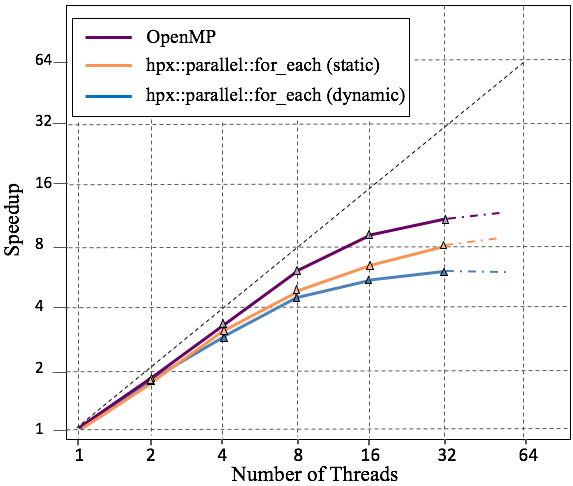
\includegraphics[width=1\columnwidth]{Pictures/parallel_for_each.jpg}
\caption {\small{Comparison results of strong scaling between \texttt{\#pragma omp parallel for} and \texttt{hpx::parallel::for\_each} with dynamic and static \texttt{chunk\_size} used for an Airfoil application
with up to 64 threads. HPX allows controlling a grain size while using \texttt{hpx::parallel::for\_each} to improve scalability. The results illustrate a better performance for \texttt{hpx::parallel::for\_each} with the static \texttt{chunk\_size} compared to the dynamic \texttt{chunk\_size} for small loops. However, OpenMP performs better than HPX in this example.}}
\label{f1}
\end{center}
\end{figure}


\begin{figure} 
\begin{center}
\centering
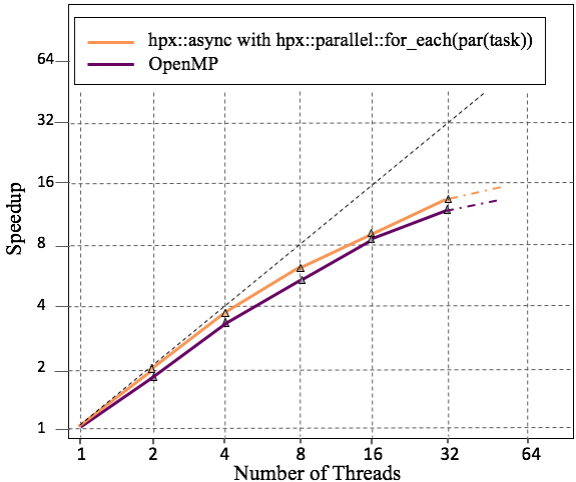
\includegraphics[width=1\columnwidth]{Pictures/async.jpg}
\caption {\small{Comparison results of strong scaling between \texttt{\#pragma omp parallel for} and \texttt{hpx::async} used for Airfoil application
with up to 64 threads. The results illustrate a better performance for \texttt{hpx::async} for the larger number of threads, which is due to the asynchronous task execution provided with a returned $future$. }}
\label{f3}
\end{center}
\end{figure}

\begin{figure} 
\begin{center}
\centering
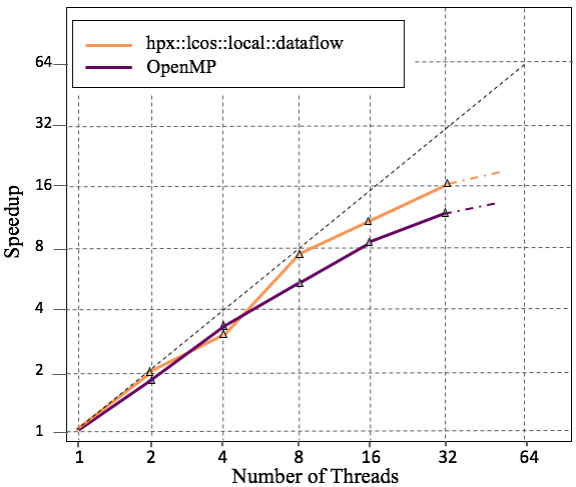
\includegraphics[width=1\columnwidth]{Pictures/dataflow.jpg}
\caption {\small{Comparison results of strong scaling between \texttt{hpx::lcos::local::dataflow} and \texttt{\#pragma omp parallel for} used for Airfoil application
with up to 64 threads. The results illustrate a better performance for \texttt{hpx::lcos::local::dataflow} for the larger number of threads, which is due to the asynchronous task execution. \texttt{hpx::lcos::local::dataflow} automatically generated an execution tree, which represents a dependency graph and allows to execute a function asynchronously. }}
\label{f2}
\end{center}
\end{figure}
 

For evaluating HPX performance for loop parallelization produced with OP2, we perform the strong scaling experiments and weak scaling experiments. For studying speedup, we use strong scaling, for which the problem size is kept the same as the number of threads increases. Figure \ref{f1} shows the strong scaling for these three loop parallelization methods: \texttt{\#pragma omp parallel for} and \texttt{hpx::parallel::for\_each} with dynamic and static \texttt{chunk\_size} for an Airfoil application explained in section \ref{sec:for}. As discussed in section \ref{sec:for}, HPX allows controlling a grain size at runtime while using \texttt{hpx::parallel::for\_each} to improve scalability. Figure \ref{f1} illustrates that \texttt{hpx::parallel::for\_each} with the static \texttt{chunk\_size} has a better performance compared to the dynamic \texttt{chunk\_size}, which is due to the small execution time of the loops compared to the total execution time of an Airfoil application. But, it can be seen that OpenMP still performs better than HPX in this example.



Figure \ref{f3} shows the strong scaling comparison results for \texttt{\#pragma omp parallel for} and \texttt{hpx::async} from \ref{sec:async}. It shows a better performance for \texttt{hpx::async}, which is a result of asynchronous execution of loops provided with returned $future$s.


Figure \ref{f2} shows the strong scaling comparison results for \texttt{\#pragma omp parallel for} and \texttt{hpx::lcos::local::dataflow}. \texttt{hpx::parallel::for\_each} is used for the loop parallelization \texttt{hpx::lcos::local::dataflow} as discussed in Section \ref{sec:with}. Figure \ref{f2} illustrates a better performance for \texttt{hpx::lcos::local::dataflow} which is due to the asynchronous task execution. \texttt{hpx::lcos::local::dataflow} automatically generated an execution tree, which represents a dependency graph and allows to execute a function asynchronously. Asynchronous task execution removes a global barrier synchronization after each loop and as a results improves a scalability for a parallel applications.    

By considering the above results, we can see the improvement in the performance over the OP2 (initial) version. For $32$ threads in Figure \ref{f3}, \texttt{hpx::async} improves a scalability by about 5\% and in Figure \ref{f2}, \texttt{hpx::lcos::local::dataflow} improves a scalability by about 27\% and compared to \texttt{\#pragma omp parallel for}. These results show a good scalability achieved by HPX and indicates that it has the potential to continue to scale on more number of threads.

To study the effects of communication latencies, we perform weak scaling experiments, where the problem size is increased in proportion to the increase of the number of cores. Figure shows a weak scaling of using \texttt{\#pragma omp parallel for}, \texttt{hpx::parallel::for\_each}, \texttt{hpx::async} and \texttt{hpx::lcos::local::dataflow} for a loop parallelization. It can be seen when the problem size is large enough, there will be enough work for all threads, which hides the communication latencies behind useful work. So for the larger problem size, the more parallelism can be extracted from the application which results to the better parallel efficiency. 


\begin{figure} 
\begin{center}
\centering
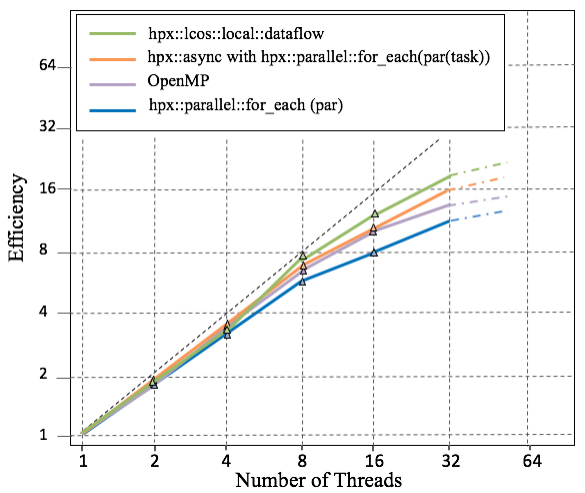
\includegraphics[width=1\columnwidth]{Pictures/weak.jpg}
\caption {\small{Comparison results of a weak scaling between \texttt{\#pragma omp parallel for}, \texttt{hpx::parallel::for\_each}, \texttt{hpx::async} and \texttt{hpx::lcos::local::dataflow} used for Airfoil application
with up to 64 threads. The results illustrate a better performance for \texttt{hpx::lcos::local::dataflow} for the larger number of threads, which shows
the perfect overlap of computation with communication enabled by HPX.}}
\label{f2}
\end{center}
\end{figure}






\section{Conclusion}
\label{sec:future}

The work presented in this paper shows how the HPX runtime system can be used to implement C++ application frameworks. We changed the OP2 python source-to-source translator to automatically use HPX for loop parallelization within a code generated by OP2. Airfoil simulation written in OP2 is used to compare the HPX performance with OpenMP that is used in OP2 parallel loops. We were able to obtain 27\% scalability improvement in using \texttt{hpx::lcos::local::dataflow} for loop parallelization compared with OpenMP.

With using \texttt{hpx::parallel::for\_each}, HPX is able to control a grain size at runtime and as a result the resource starvation is reduced as well. However, using \texttt{hpx::parallel::for\_each} introduces the global barriers at the end of the loop same as OpenMP, which inhibits having a desired scalability. On the other hand, \texttt{hpx::lcos::local::dataflow} allows the computation within a loop to be processed as far as possible, which avoids a global barrier synchronization. \texttt{hpx::lcos::local::dataflow} gives a capability of automatically interleaving consecutive loops during a runtime, which they do not need to wait for the previous loops to be completed. OP2 API is modified to take full advantage of all available parallel resources through HPX. It was illustrated that a returned $future$ from each function within \texttt{op\_par\_loop} removes the necessitate of having a barrier at the end of each loop and results in significantly improving a parallelism level.





 


\bibliography{References}
\bibliographystyle{IEEEtran}


\end{document}

